\documentclass{article}
\usepackage[utf8]{inputenc}
\usepackage{graphicx}

\title{Membuat Aplikasi Di Oracle APEX}
\author{ayuanandra4 }
\date{07 November 2019}

\begin{document}

\maketitle

\section{Langkah-Langkah Membuat Aplikasi Di Oracle Apex}

\begin{enumerate}
    \item {Langkah pertama kita masuk ke link untuk masuk ke oracle apex online https://apex.oracle.com/pls/apex/f?p=4550:1:101898625730364:::::, kemudian login dengan memasukan Workspace, Ussername, dan Password}
  \begin{center}
        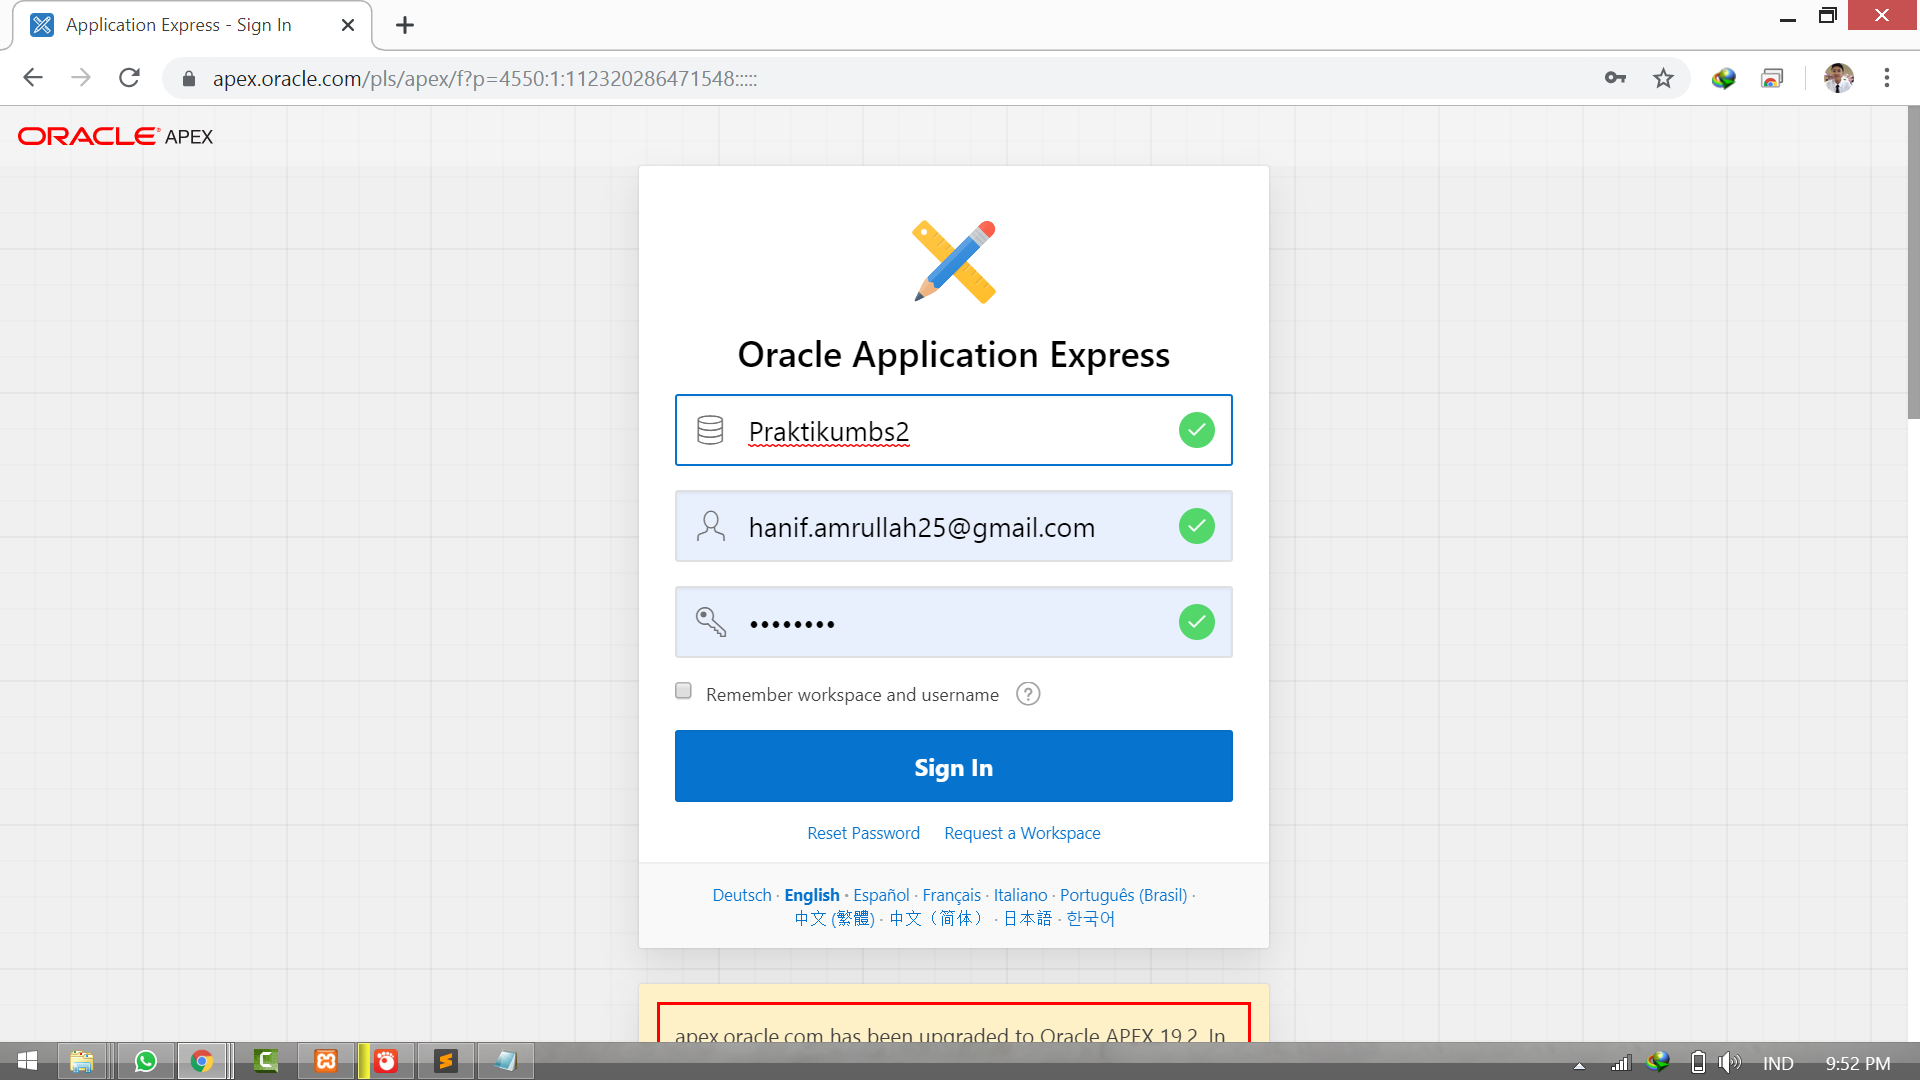
\includegraphics[width = 10cm\textwidth]{1.png}
    \end{center}
    
    \item {Setelah login, masuk ke halaman utama dan pilih create}
    \begin{center}
        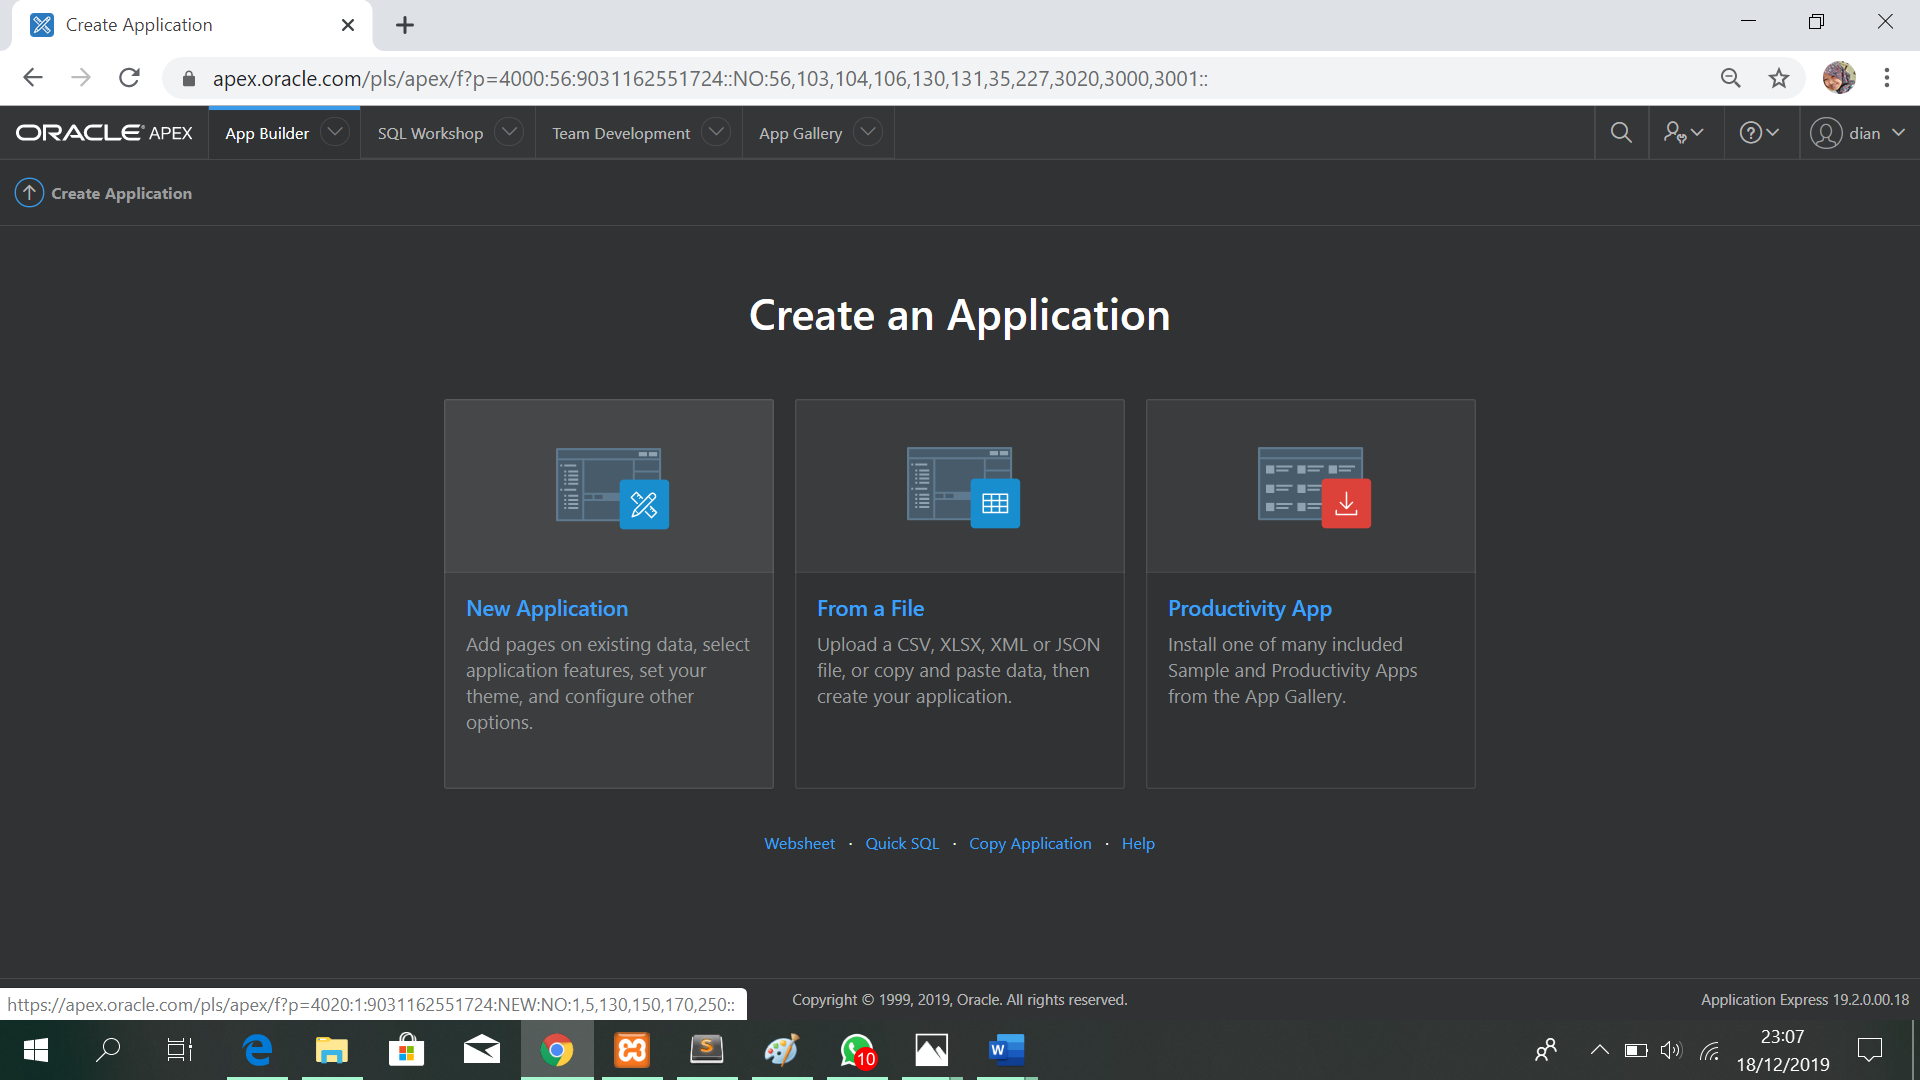
\includegraphics[width = 10cm\textwidth]{2.png}
    \end{center}
    
    \item {Langkah selanjutnya pilih Form a File}
    \begin{center}
        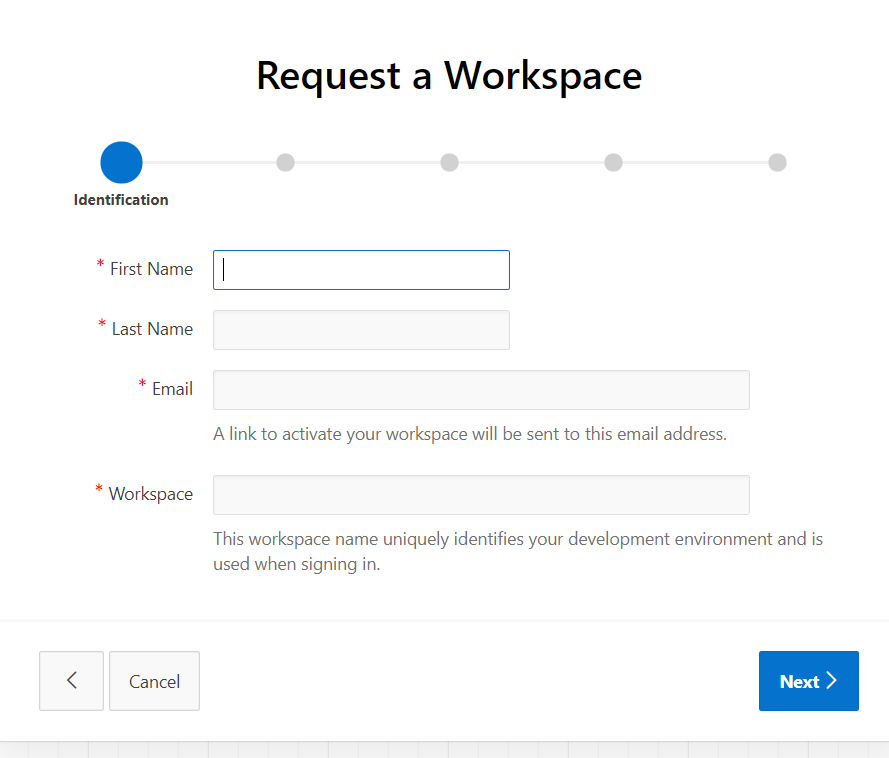
\includegraphics[width = 10cm\textwidth]{3.png}
    \end{center}

    \item {Kemudian pilih file dari laptop yang telah kita buat terlebih dahulu}
    \begin{center}
        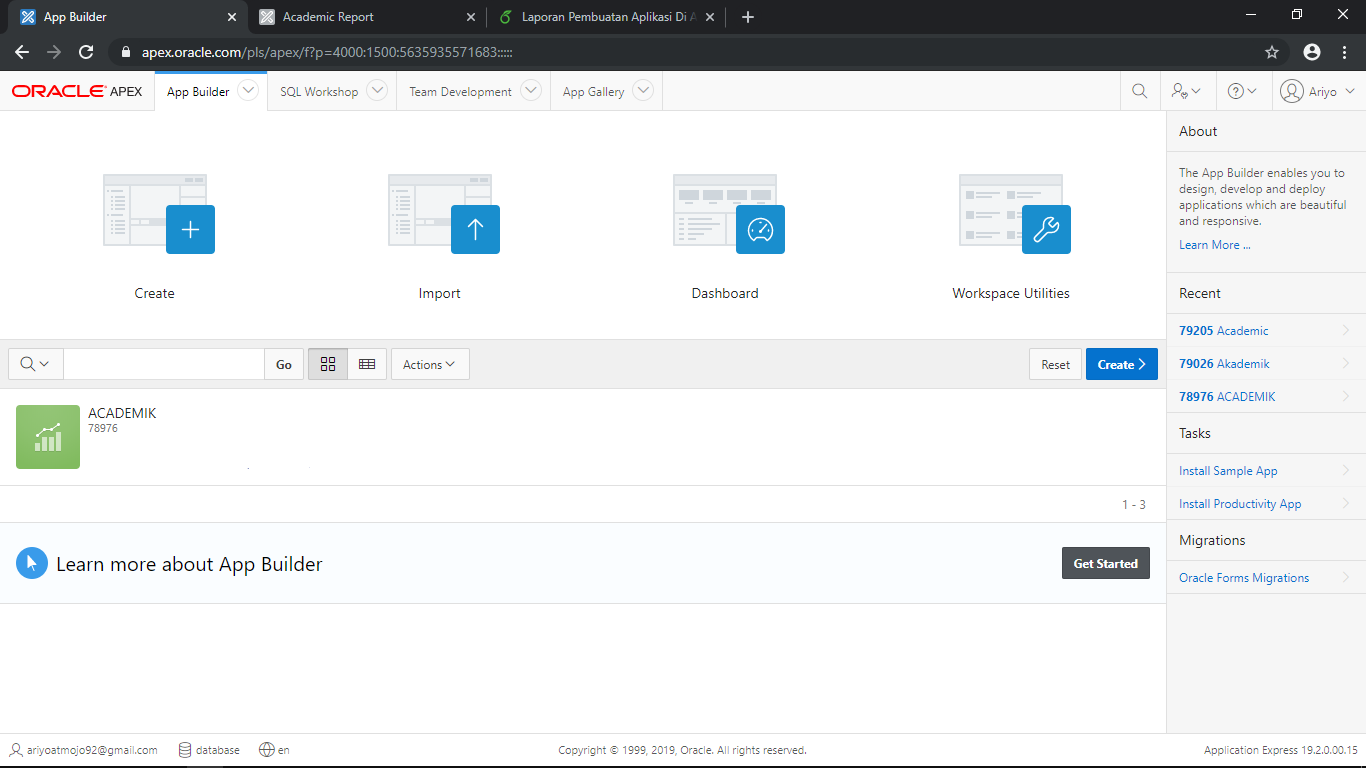
\includegraphics[width = 10cm\textwidth]{4.png}
    \end{center}
    
    \item {Selanjutnya mengisi nama table dan klik load data}
    \begin{center}
        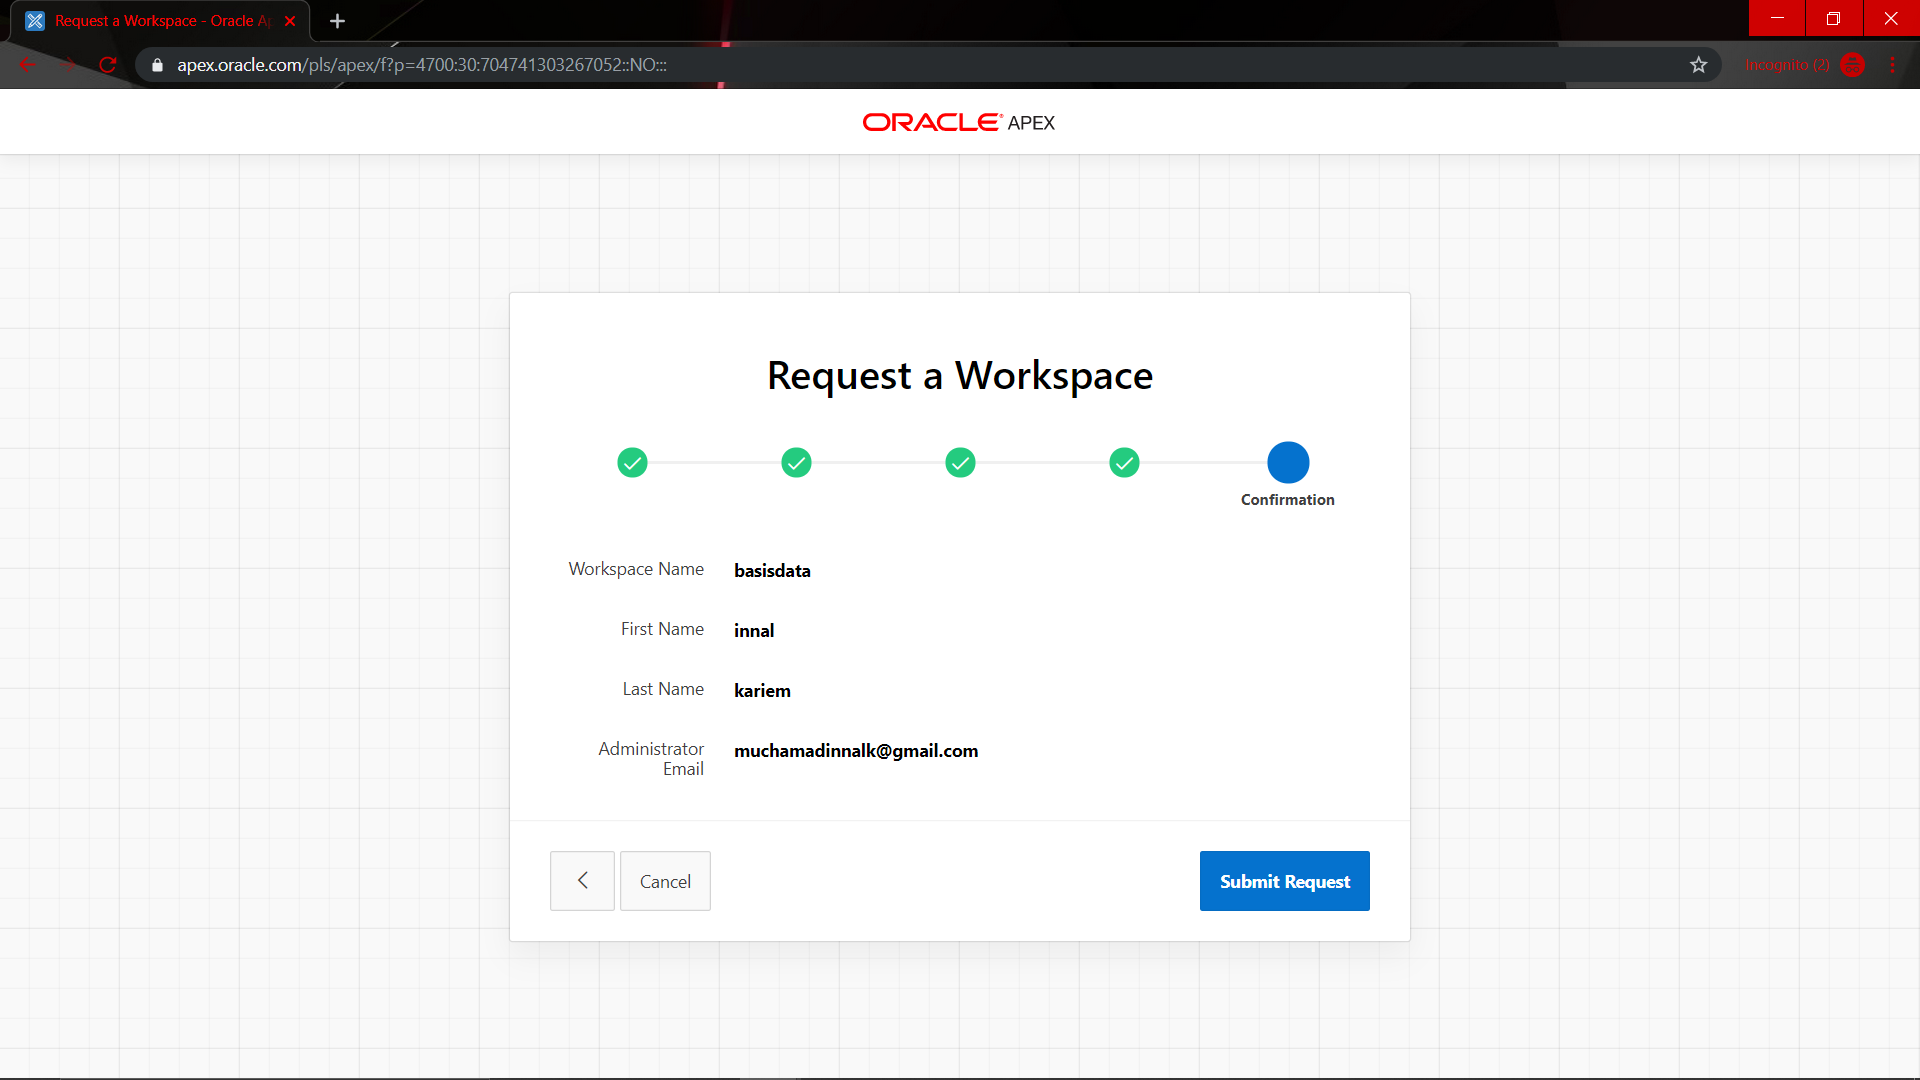
\includegraphics[width = 10cm\textwidth]{5.png}
    \end{center}
    
    \item {Setelah mengklik load data jika berhasi, gambar nya akan seperti dibawah ini}
    \begin{center}
        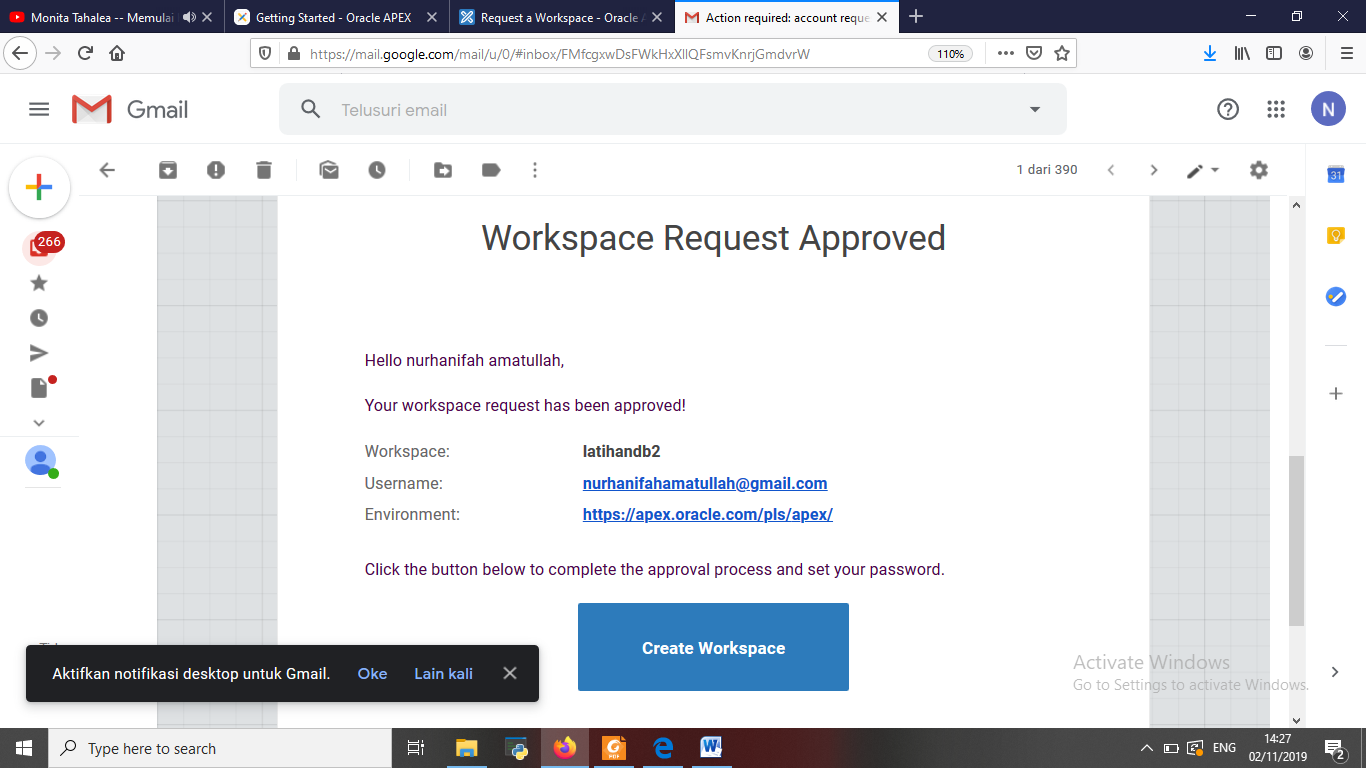
\includegraphics[width = 10cm\textwidth]{6.png}
    \end{center}

    \item {Setelah semua data yang akan kita buat diinputkan, Primary key (ID) yang ada di table di hapus}
    \begin{center}
        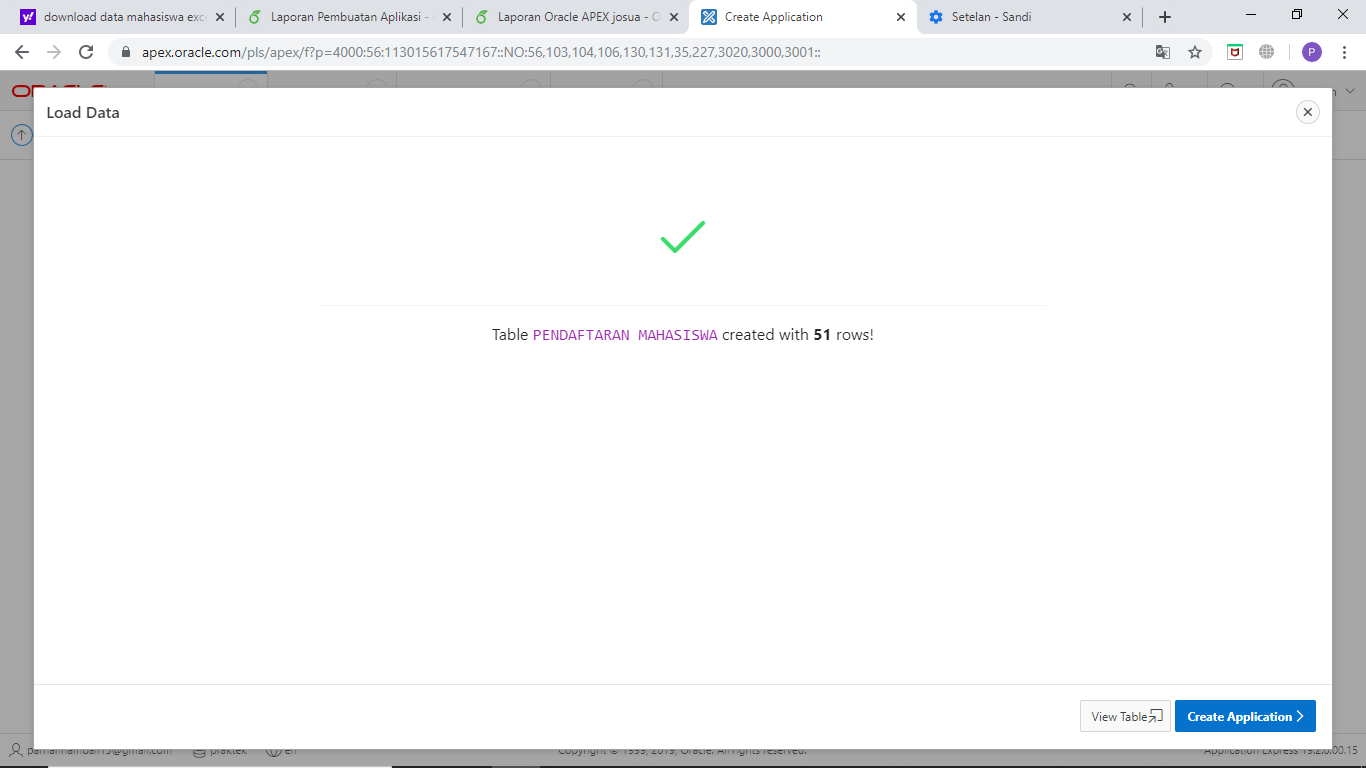
\includegraphics[width = 10cm\textwidth]{8.png}
    \end{center}
    
    \item {Menuliskan Query untuk menambahkan primary key dan foreign key}
     \begin{center}
        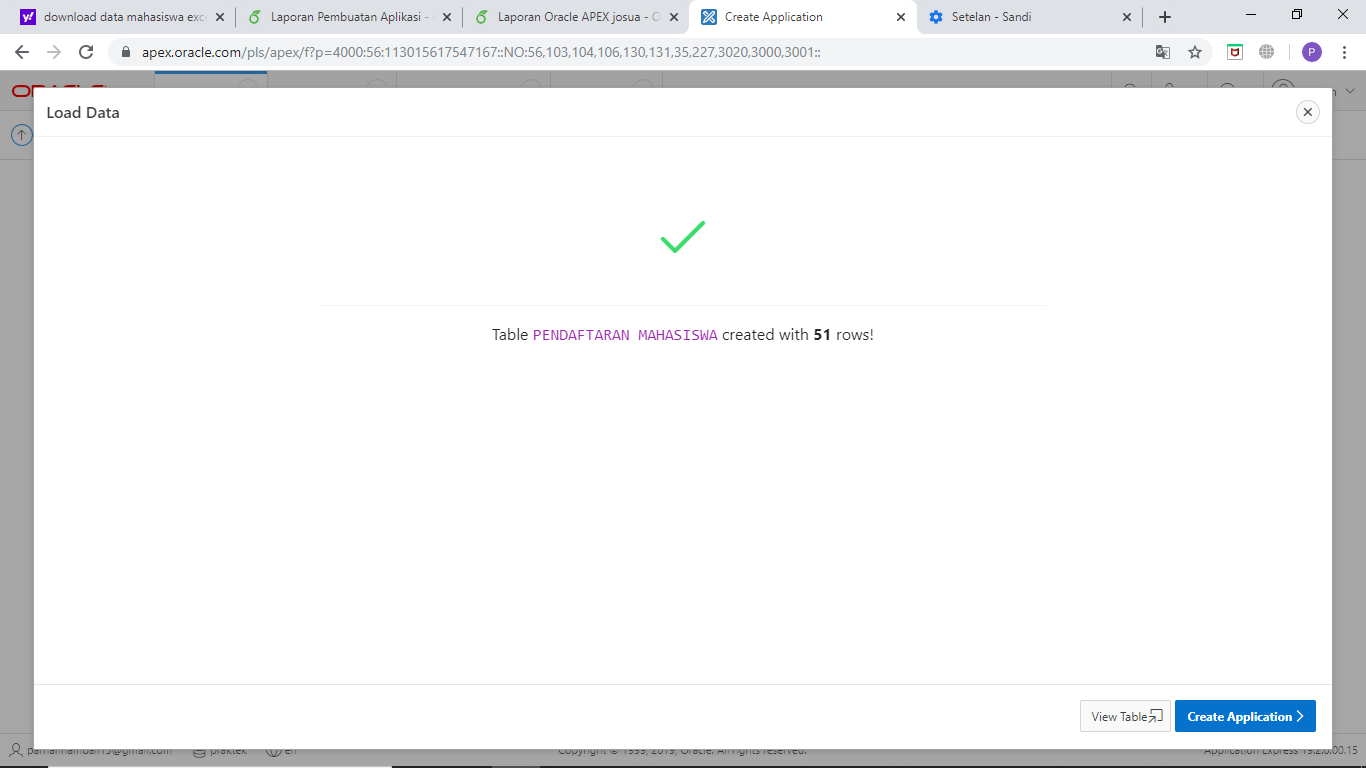
\includegraphics[width = 10cm\textwidth]{8.png}
    \end{center}
     
    \item {Jika data sudah dipastikan sesuai dengan primary key dan foreigen key, maka buat aplikasinya. Klik App Build, Klik create, Pilih New Application. Dan inputkan tabel tabel yang lain nya}
    \begin{center}
        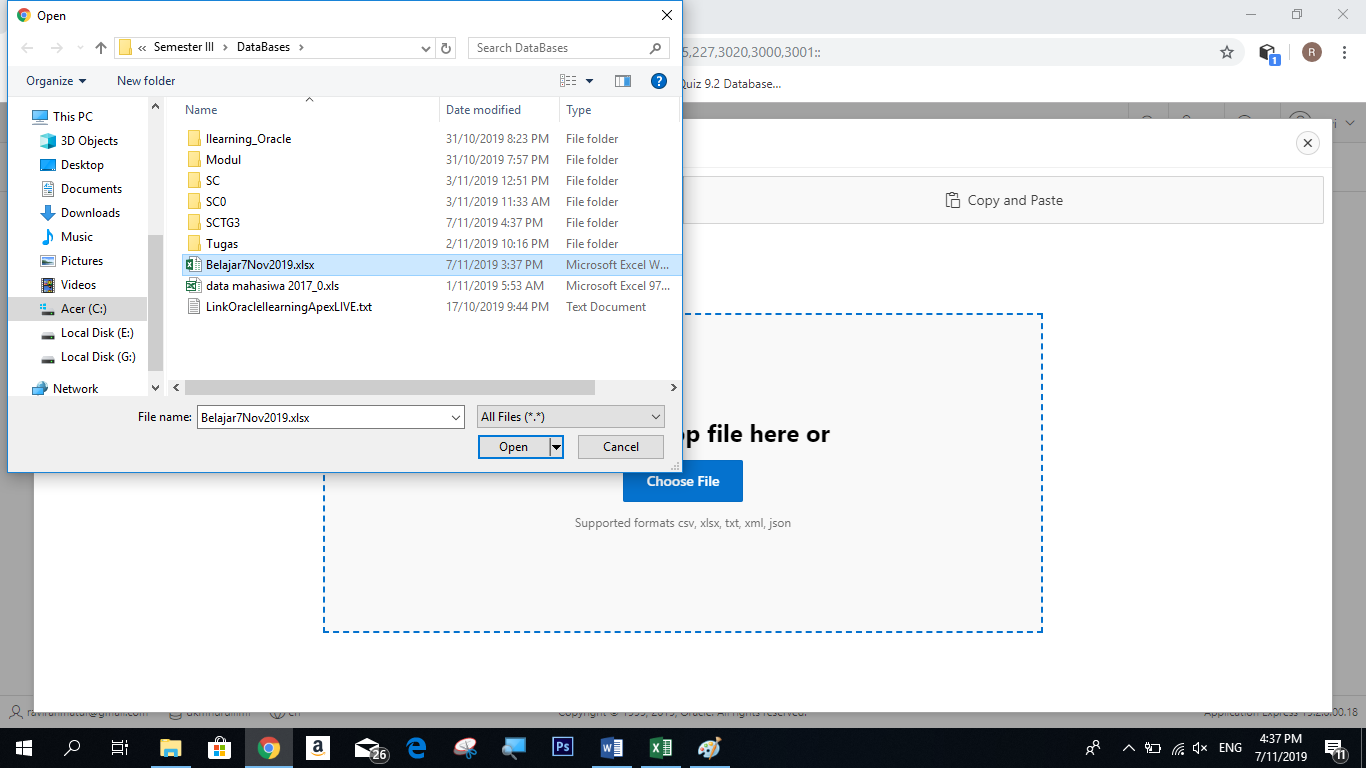
\includegraphics[width = 10cm\textwidth]{9.png}
     \end{center}
     
    \item {Setelah Muncul Create an Application, Klik Add Page untuk memilih tampilan halaman, lalu Create Form Page untuk memilih table mana yang akan di tambahkan}
     \begin{center}
        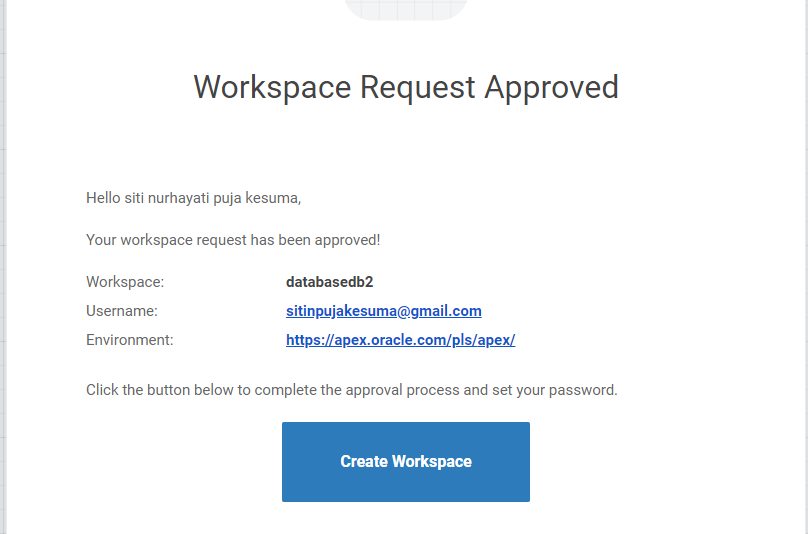
\includegraphics[width = 10cm\textwidth]{10.png}
    \end{center}
    
     \begin{center}
        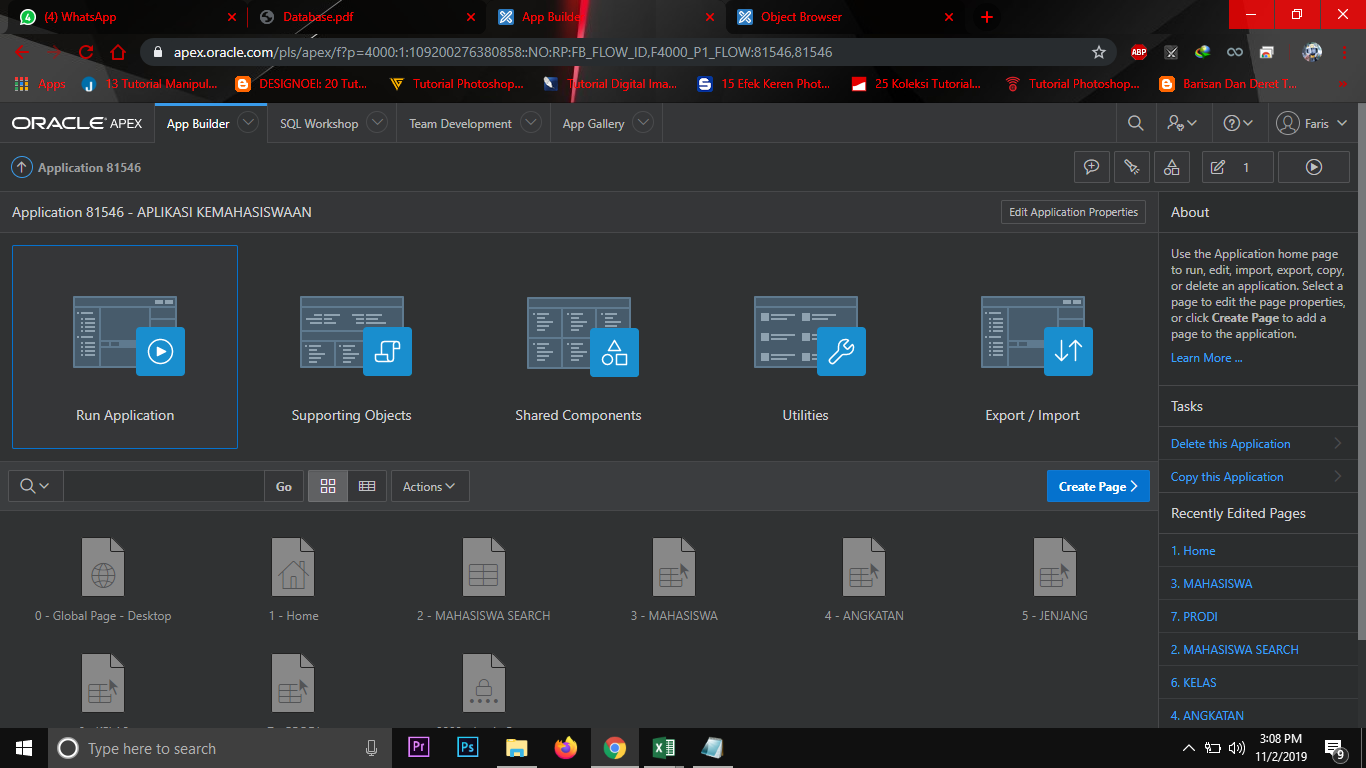
\includegraphics[width = 10cm\textwidth]{11.png}
    \end{center}
    
    \item {Langkah berikutnya Run Application yang telah di buat}
    \begin{center}
        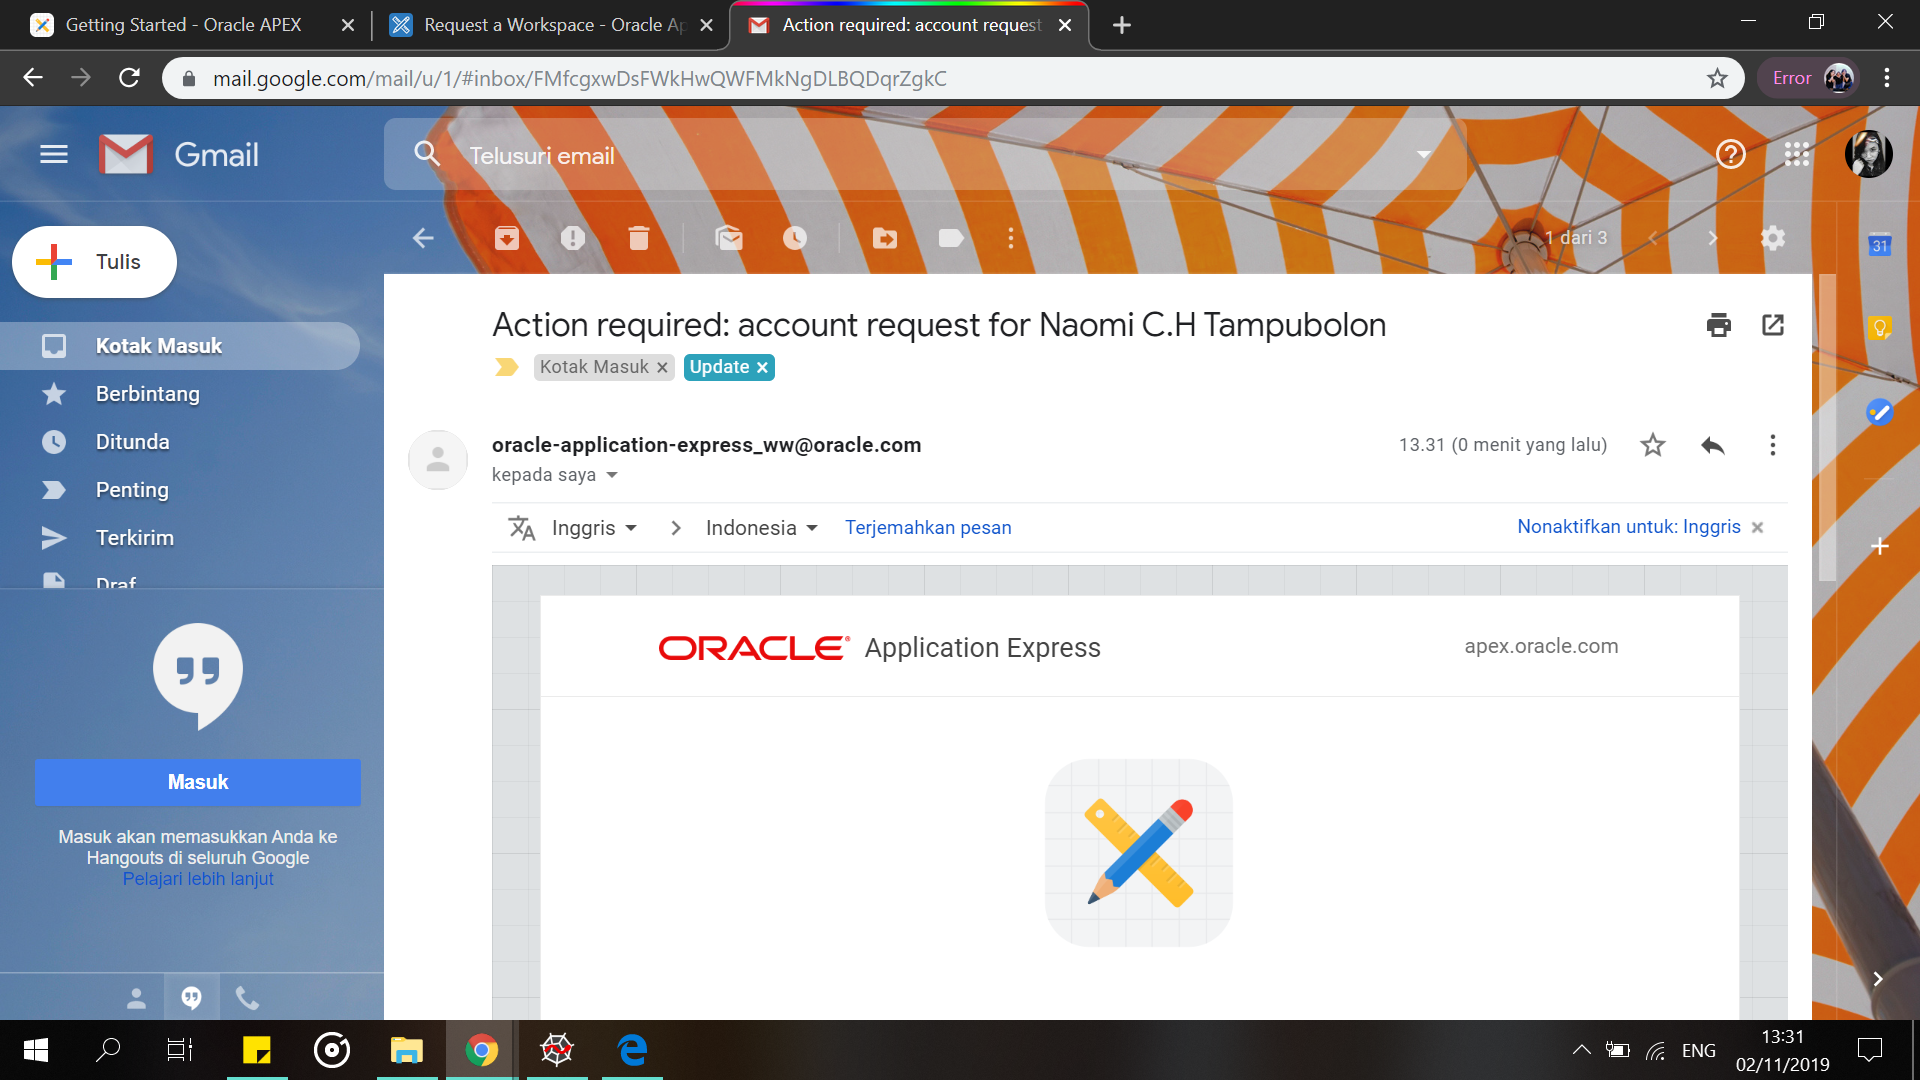
\includegraphics[width = 10cm\textwidth]{13.png}
    \end{center}
    
    \item {Login ke applikasi yang telah kita buat dengan masukkan link https://apex.oracle.com/pls/apex/f?p=93063:LOGIN_DESKTOP:104427093459928:::::, dengan Username : AYUANANDRA4@GMAIL.COM dan Password : anandra4} 
    \begin{center}
        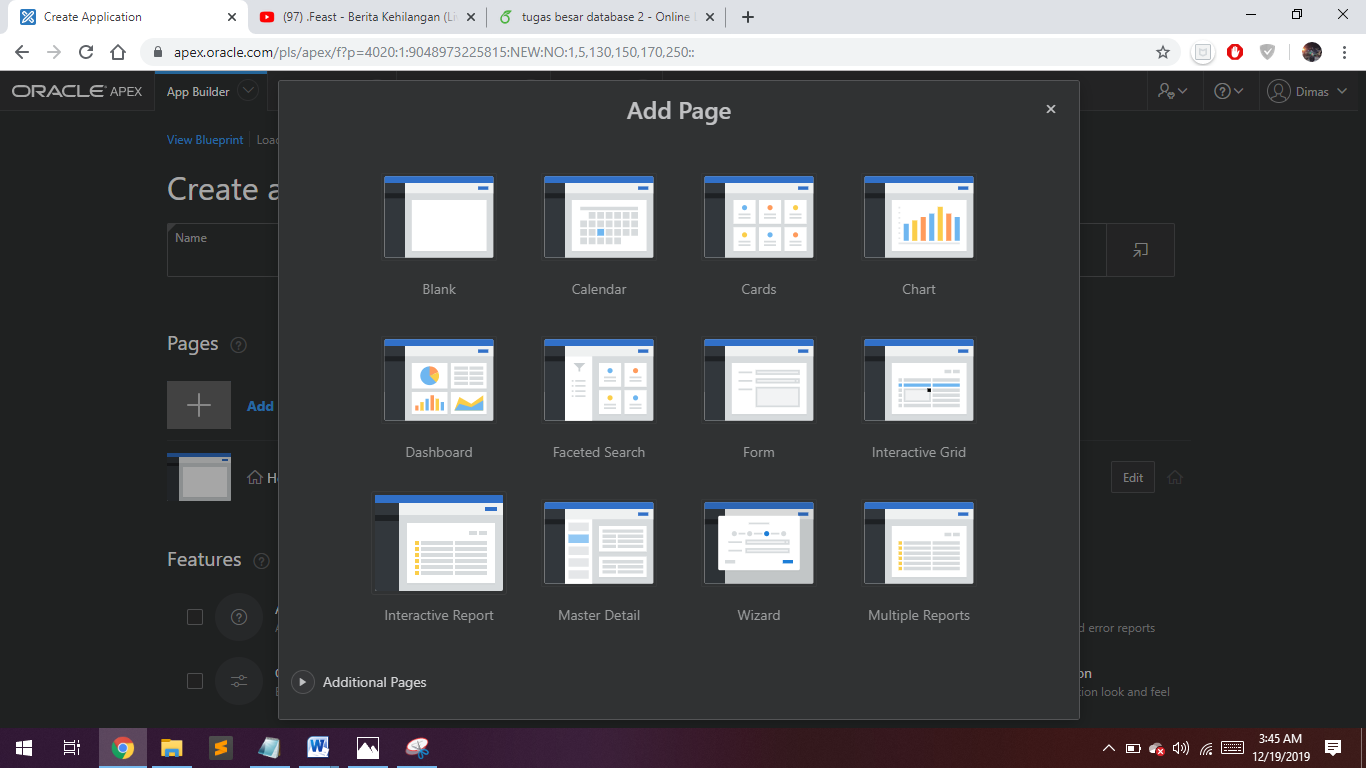
\includegraphics[width = 10cm\textwidth]{14.png}
    \end{center}
    
    \item {Gambar di bawah ini merupakan tampilan dari applikasinya}
    \begin{center}
        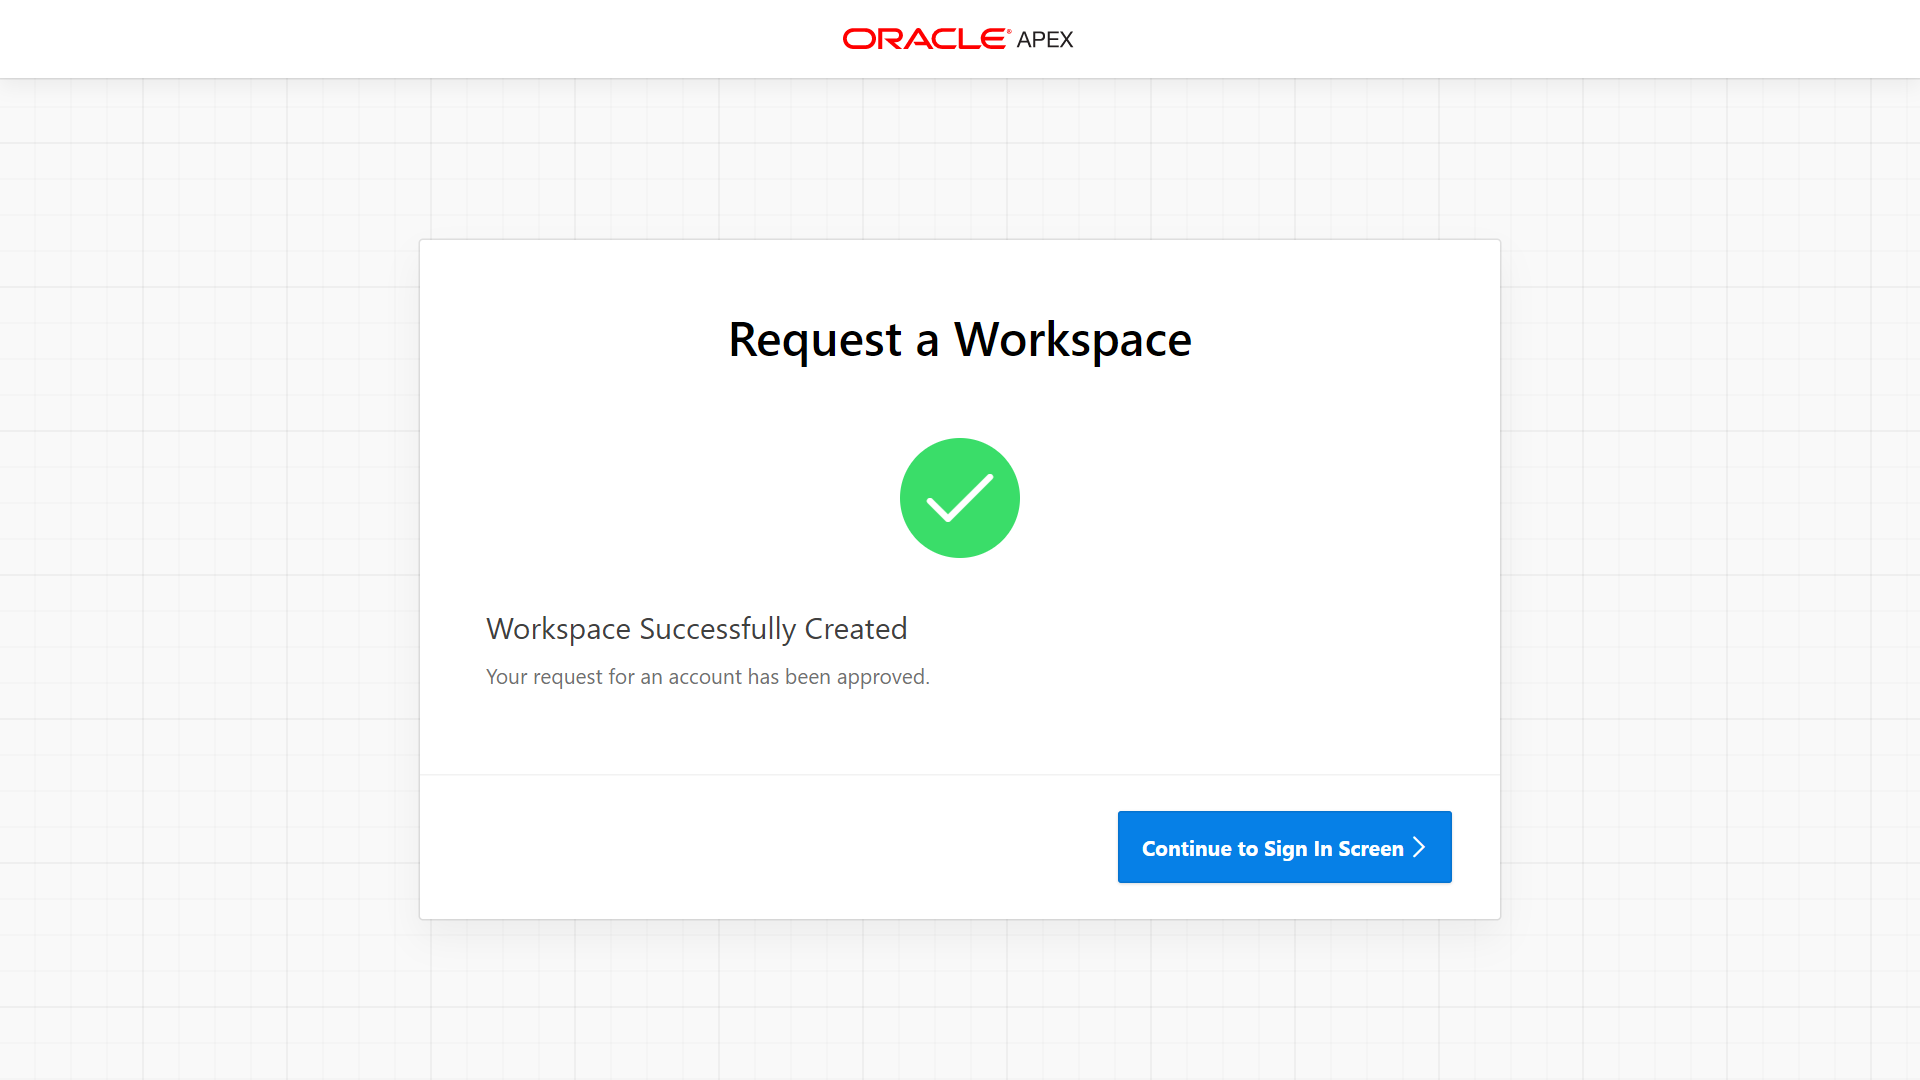
\includegraphics[width = 10cm\textwidth]{15.png}
    \end{center}
    
    \end{enumerate}
\end{document}
